% Created 2022-08-25 jue 11:39
% Intended LaTeX compiler: pdflatex
\documentclass[12pt]{article}
\usepackage[utf8]{inputenc}
\usepackage[T1]{fontenc}
\usepackage{graphicx}
\usepackage{grffile}
\usepackage{longtable}
\usepackage{wrapfig}
\usepackage{rotating}
\usepackage[normalem]{ulem}
\usepackage{amsmath}
\usepackage{textcomp}
\usepackage{amssymb}
\usepackage{capt-of}
\usepackage{hyperref}
\usepackage[spanish]{babel}
\usepackage{graphicx,geometry}
\geometry{ a4paper, left=1in, right=1in, top=1in, bottom=1in }
\renewcommand\familydefault{\sfdefault}
\usepackage{sectsty}
\sectionfont{\normalfont\large }
\usepackage{tabularx}
\usepackage{listings}
\lstdefinestyle{mystyle}{
numbers=left,
showspaces=false,
frame=leftline,
showspaces=false,
showstringspaces=false,
showtabs=false,
numberstyle=\tiny,
}
\lstset{
style=mystyle,
literate={á}{{\'a}}1
{é}{{\'e}}1
{í}{{\'{\i}}}1
{ó}{{\'o}}1
{ú}{{\'u}}1
{Á}{{\'A}}1
{É}{{\'E}}1
{Í}{{\'I}}1
{Ó}{{\'O}}1
{Ú}{{\'U}}1
{ü}{{\"u}}1
{Ü}{{\"U}}1
{ñ}{{\~n}}1
{Ñ}{{\~N}}1
{¿}{{?``}}1
{¡}{{!``}}1
}
\makeatletter
\usepackage{fancyhdr}
\pagestyle{fancy}
\usepackage{mdframed}
\BeforeBeginEnvironment{minted}{\begin{mdframed}}
\AfterEndEnvironment{minted}{\end{mdframed}}
\author{Luis Eduardo Galindo Amaya (1274895)}
\date{2022-08-23}
\title{Exploración de los Componentes de un Entorno de Desarrollo Integrado}
\hypersetup{
 pdfauthor={Luis Eduardo Galindo Amaya (1274895)},
 pdftitle={Exploración de los Componentes de un Entorno de Desarrollo Integrado},
 pdfkeywords={},
 pdfsubject={},
 pdfcreator={Emacs 26.3 (Org mode 9.1.9)}, 
 pdflang={Spanish}}
\begin{document}


\newcommand{\docente}{Manuel Castañón-Puga}
\newcommand{\asignatura}{Herramientas de Desarrollo de Software (40017)}
\newcommand{\semestre}{2022-2}

\newcommand{\miportada}[1]{
	\begin{titlepage}
		\vspace*{0.75in}
		\begin{flushleft}
			\sffamily
			\large #1       \\
			\Huge 
            \@title         \\
			\hrulefill
			\vspace{0.25in} \\
			\Large \@author \\
			\vspace*{\fill}
            
\includegraphics[width=\textwidth]{../includes/filler.png} \\
			\vspace*{\fill}
			\large
			\begin{tabular}{|l|l|}
              \hline
			  Asignatura & \asignatura \\
			  Docente    & \docente    \\
			  Fecha      & \@date      \\
              \hline
			\end{tabular}
		\end{flushleft}
	\end{titlepage}
}

\fancyhf{}
\lhead{ \asignatura }
\rhead{ \semestre }
\rfoot{Página \thepage}

\setlength\parindent{0pt}   % eliminar el intentado
\setlength{\parskip}{1.2em}
% \maketitle

\thispagestyle{empty}
\begin{center}
	{\large
		UNIVERSIDAD AUTÓNOMA DE BAJA CALIFORNIA \\
		Facultad de Ciencias Químicas e Ingeniería }
	\vspace{0.25in} \\
	Programa de Ingeniero en Software y Tecnologías Emergentes
\end{center}

\section*{Información De La Materia}
\label{sec:org7f9e35c}
\begin{mdframed}
\begin{description}
\item[{Asignatura}] \asignatura .
\item[{Grupo y Periodo}] 341 (2022-2) .
\item[{Docente}] \docente .
\end{description}
\end{mdframed}

\section*{Información De La Actividad}
\label{sec:orgac31032}
\begin{mdframed}
\begin{description}
\item[{Nombre de la actividad}] Práctica de laboratorio 1.1.1: Instalación y configuración de entorno de desarrollo integrado.
\item[{Fecha}] 2022-08-23
\item[{Lugar}] Edificio 6E, Salón 204.
\item[{Carácter de la actividad}] Individual.
\item[{Participante(es)}] Luis Eduardo Galindo Amaya (1274895).
\end{description}
\end{mdframed}

\section*{Reporte De Actividades}
\label{sec:org3085093}
\subsection*{Eclipse}
\label{sec:org828d822}
\begin{figure}[htbp]
\centering
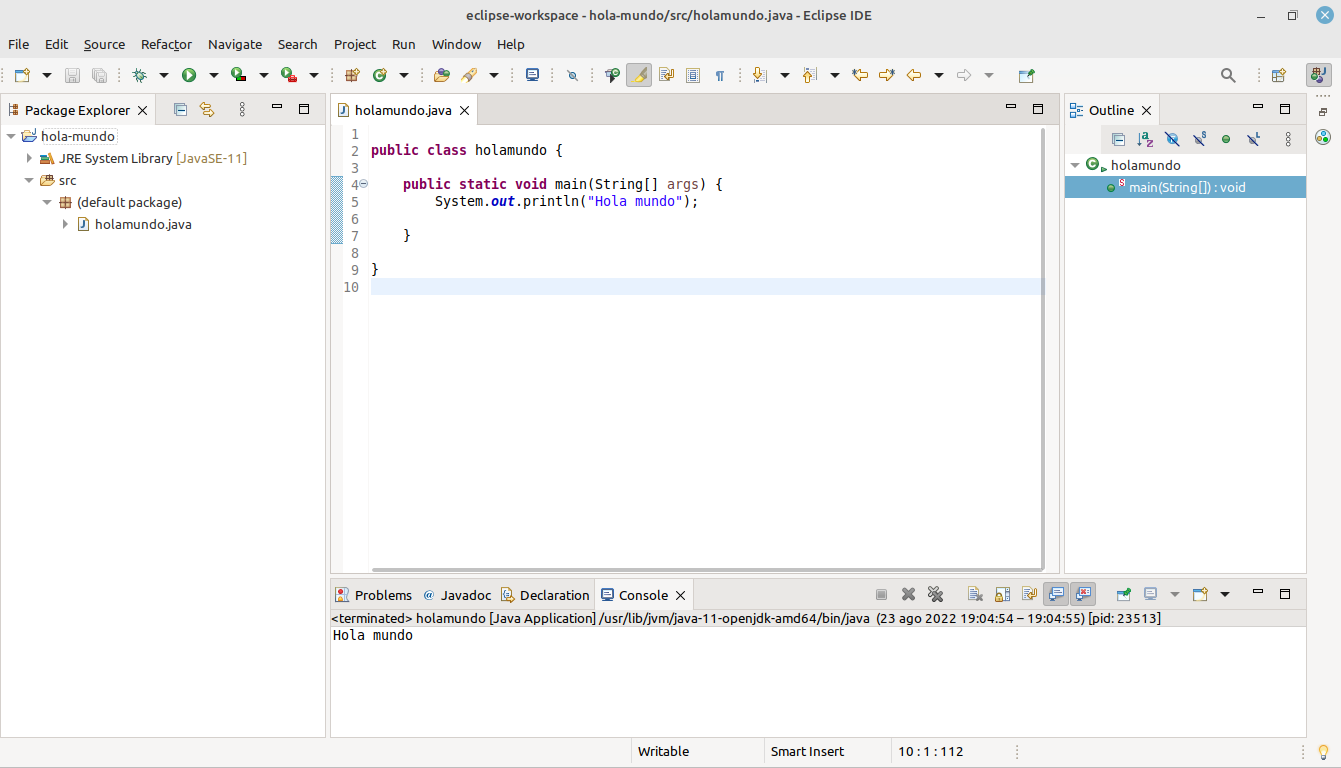
\includegraphics[width=7.5cm]{./img/eclipse.png}
\caption{'Hola mundo' en Java, Eclipse IDE}
\end{figure}

El editor mas veterano de los tres, el estilo de la interfaz es muy propio del software empresarial y conociendo que todavía es parte de algunas de las suites de herramientas de IBM no es nada de lo que hay que sorprenderse.

Los plugins en Eclipse son mas escasos que en otras herramientas y se sienten mas como algo que pusieron después que como algo con lo que se planeo el editor. 

Las herramientas para refactorización de código son un poco mas complicadas de usar, aunque no tuve tanto tiempo para probarlas como me gustaría. El auto completado es bueno, pero no pasa de simplemente mostrar que cosas se encuentran dentro de que paquetes, otros IDEs para java suelen mostrar la documentación de cada función auque imagino que es posible activar esta función en algún lugar o con algún plugin.  

\subsection*{Pycharm}
\label{sec:org420966b}
Se siente muy robusta y tiene una interfaz muy moderna, siento que cumple todo lo que un IDE debería tener: herramientas de refactorizacion, plugins, auto completado, herramientas para hacer debugging etc. La única critica que podría hacer es que es demasiado lento, usualmente los IDEs son muy lentos pero particularmente los producto de Intellij son particularmente lentas, el catalogo de plugins también es un poco pequeño a comparación de otros editores.

\begin{figure}[htbp]
\centering
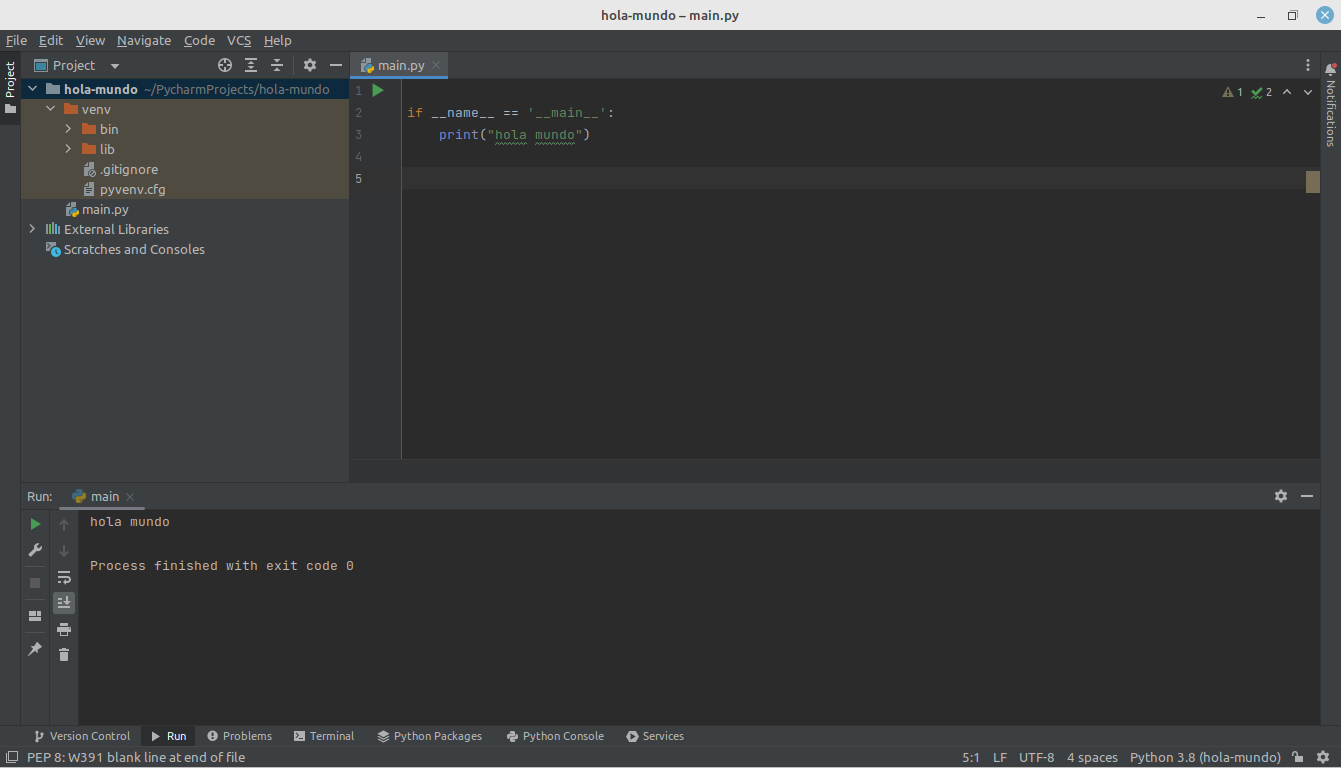
\includegraphics[width=7.5cm]{./img/pycharm.png}
\caption{'Hola mundo' en Python, Pycharm IDE}
\end{figure}


\subsection*{Visual Estudio Code}
\label{sec:org592bdaa}
La apuesta de Microsoft en los editores de código, a comparación de Eclipse y pycharm no tiene casi herramientas montadas con el editor sin embargo a pesar de eso puede obtener esta funcionalidad por medio de su sistema de plugins que sin duda es el mas amplio de los tres, hay plugins de herramientas muy especificas y soporte para casi todos los lenguajes existentes desde c hasta elixir, VS-Code es una alternativa mas ligera pero con menos funcionalidad fuera de la caja y esta en manos del usuario convertir VS-Code en algo que sea funcional para su trabajo.

\begin{figure}[htbp]
\centering
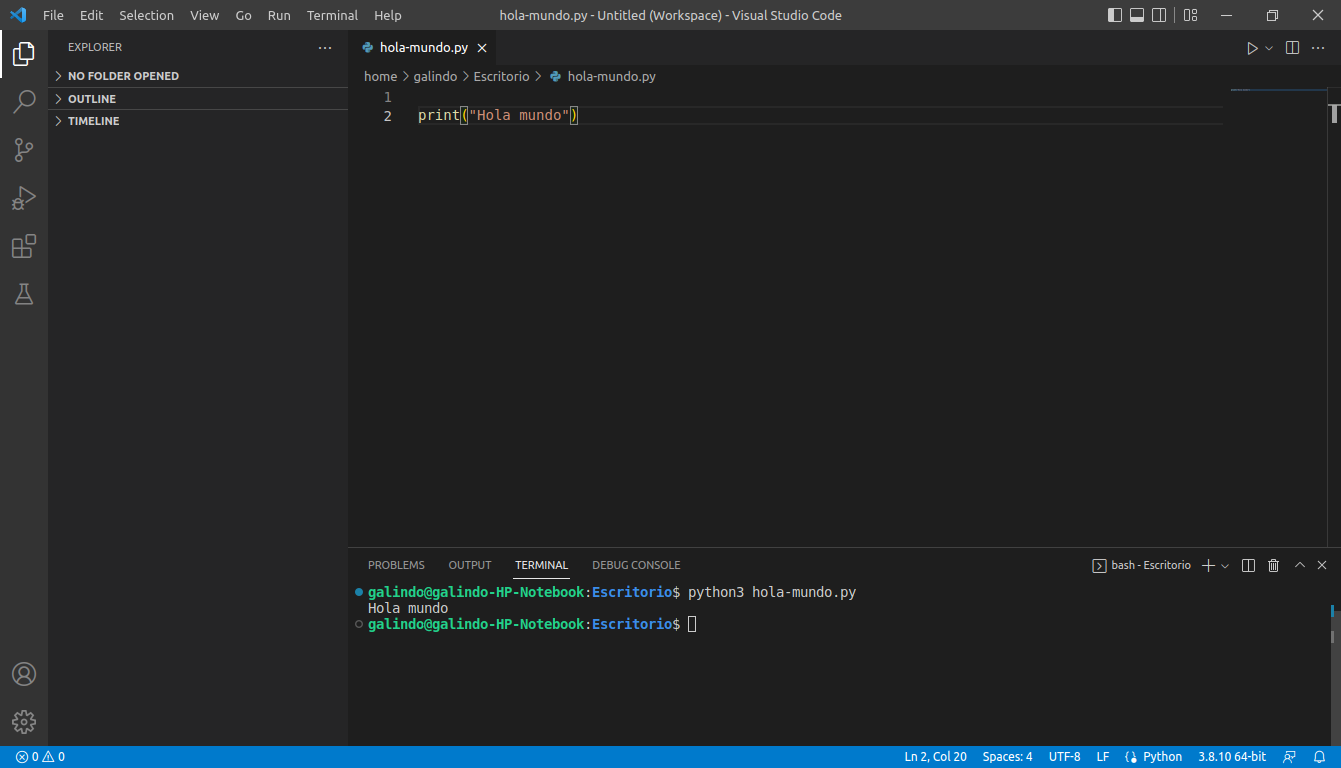
\includegraphics[width=7.5cm]{./img/visual-studio.png}
\caption{'Hola mundo' en Python, Visual studio code}
\end{figure}

\pagebreak

\section*{Reflexión}
\label{sec:org417f437}
\begin{mdframed}
En mi opinión a comparación de los editores de texto tradicionales los IDEs son herramientas muy pesas y muy complejas para cualquier edición casual de código sin embargo ese no es su objetivo, la principal ventajas de un IDE es unificar todas las herramientas que un desarrollador pude llegar a utilizar permite cierto entendimiento común entre los integrantes del equipo sin importar que tan experimentados sean con el lenguaje todos tienen a su disposición las herramientas necesarias para poder ser productivos.
\end{mdframed}

\begin{center}
Doy fe de que toda la información dada es  completa y correcta. \\
\begin{center}

\includegraphics[width=3cm]{../includes/firma.png}
\end{center}
Luis Eduardo Galindo Amaya (1274895)
\end{center}
\end{document}
